\subsection{Estudio técnico}

\subsubsection*{Tamaño}
Según el decreto 957 de 05 de junio de 2019 se presentan los criterios de clasificación de las micro, pequeñas, medianas y grandes empresas, con este presentamos una clasificación del tamaño empresarial según la ley colombiana según las variables de ingresos y costos relacionadas. También se determina el tamaño inicial de la compañía al limitar sus servicios a nivel distrital y bajo el estudio de mercado desarrollado se tendrán las acciones pertinentes para el crecimiento y desarrollo del producto, considerando factores como:

\begin{itemize}
    \item Recursos Humanos: La compañía cuenta con una estructura organizacional donde se presentan departamentos administrativos, marketing, ventas y desarrollo, para que de esta manera el recurso humano sea estratégicamente organizado para un eficiente desempeño y posterior crecimiento.
    
    \item Potencial del mercado: Actualmente es un mercado con demanda y con el desarrollo de alianzas estratégicas y planes de mercadeo se puede obtener un gran impacto, obteniendo un buen posicionamiento por la prestación del servicio.
    
    \item Factores de producción: Para el inicio de la empresa la materia prima son equipos de estándar medio, pero que sin embargo cumplen con la función para los desarrolladores y área encargada de la planificación.
\end{itemize}


\subsubsection*{Localizacion}

La localización de una empresa es uno de los factores más importantes para que el impacto del producto o servicio sea representativo y suficiente para poder ingresar al mercado y conseguir posicionamiento, esto influye en la competencia del mercado y apoya la primera etapa de crecimiento de la empresa. Sin embargo, no es necesaria una ubicación estratégica, pero sí es importante que se encuentre ubicada en Bogotá puesto que será el alcance del proyecto. Es por eso que se necesitan algunos factores útiles para que se pueda tener como primera sede.

\begin{itemize}
    \item Un lugar de fácil acceso
    \item Ambiente laboral cómodo
    \item Costo accesible
    \item Servicios de conexión a internet, electricidad y servicios sanitarios
\end{itemize}

\textbf{Lugares candidatos: } Para la elección de los lugares candidatos se tuvieron en cuenta espacios diseñados para el trabajo colaborativo con ambientes agradables y que ayudan al flujo de actividades continuas y sostenidas, actualmente los espacios como coworking cumplen con la necesidad y la infraestructura buscada además de contar con espacios donde se pueda manejar la interdisciplinariedad de las partes que comparten el ambiente de trabajo, esto permite además aportar valor al producto y mejorar las oportunidades de apoyo.

\begin{itemize}
    
    \item \textbf{Office ToGo :} Son espacios de trabajo compartido donde las pequeñas y medianas empresas, emprendedores y trabajadores independientes, tienen la oportunidad de usar espacios de trabajo equipados y organizados con todo lo necesario, además de estar en las mejores ubicaciones de Bogotá y Cajicá.
    
    \begin{adjustbox}{
            center,
            caption=[{Precios Oficinas de Office ToGo}]{Oficinas de Office ToGo. },
            label={Office},
            nofloat=table, vspace={20px}}
            {
            \begin{threeparttable}
           \begin{tabular}{|cllll|cllll|p{7cm}}
            \cline{1-10}
            \multicolumn{5}{|c|}{\cellcolor[HTML]{D9EAD3}Servicio} & \multicolumn{5}{c|}{\cellcolor[HTML]{D9EAD3}Precio x mes} &  \\ \cline{1-10}
            \multicolumn{5}{|c|}{Planes virtuales}     & \multicolumn{5}{c|}{\$ 99.000 + IVA}    &  \\ \cline{1-10}
            \multicolumn{5}{|c|}{Plan emprendedor}     & \multicolumn{5}{c|}{\$ 169.000 + IVA}   &  \\ \cline{1-10}
            \multicolumn{5}{|c|}{Oficinas gerenciales} & \multicolumn{5}{c|}{\$ 1.100.000 + IVA} &  \\ \cline{1-10}
            \multicolumn{5}{|c|}{Oficina semi-privada}  & \multicolumn{5}{c|}{\$ 850.000 + IVA}   &  \\ \cline{1-10}
            \end{tabular}%
            
            \begin{tablenotes}[para,flushleft]
                \vspace{2mm}
                \textit Nota. Fuente: OfficeToGo.com 
            \end{tablenotes}
            
            \end{threeparttable} 
            }        
    \end{adjustbox}
    \item \textbf{PaqueSoft :} Parquesoft Bogotá es un proveedor multisectorial de servicios de Tecnologías de la Información, que funciona con el apoyo de más 50 empresas de base tecnológica en Bogotá, que trabajando juntas generan una oferta de valor integral, creando soluciones de calidad, a la vanguardia con últimas tendencias digitales. Parquesoft es el Cluster de ciencia y tecnología informática más grande de Colombia y uno de los más importantes líderes en apoyo a proyectos de emprendimiento con base tecnológica.
    
    
    \begin{adjustbox}{
            center,
            caption=[{Precios Oficinas de ParqueSoft.}]{Oficinas de ParqueSoft. },
            label={ParqueSoft},
            nofloat=table, vspace={20px}}
            {
            \begin{threeparttable}
           \begin{tabular}{|cllll|cllll|p{5cm}}
            \cline{1-10}
            \multicolumn{5}{|c|}{\cellcolor[HTML]{D9EAD3}Servicio} & \multicolumn{5}{c|}{\cellcolor[HTML]{D9EAD3}Precio x mes} &  \\ \cline{1-10}
            \multicolumn{5}{|c|}{Pago Mensual}   & \multicolumn{5}{c|}{$ 96.000 / Mes - $ 1.152.000 total Año} &  \\ \cline{1-10}
            \multicolumn{5}{|c|}{Pago Semestral} & \multicolumn{5}{c|}{$ 78.000 / Mes - $ 932.000 total Año}   &  \\ \cline{1-10}
            \multicolumn{5}{|c|}{Pago Anual}     & \multicolumn{5}{c|}{$ 69.000 / Mes - $ 828.000 total Año}   &  \\ \cline{1-10}
            \end{tabular}%
            
            \begin{tablenotes}[para,flushleft]
                \vspace{2mm}
                \textit Nota. Fuente: ParqueSoft.com
            \end{tablenotes}
            \end{threeparttable} 
            }        
    \end{adjustbox}
    
    \item \textbf{Elección: } Considerando todas las ofertas disponibles de sitios en donde puede consolidarse la empresa, se ha estudiado los beneficios que trae consigo en cuanto a ubicación, servicios ofrecidos, accesibilidad, seguridad, estructura física, entre otros; Se decide como mejor elección a Parquesoft ya que sus servicios son los apropiados para la compañía que recién está surgiendo, sus precios son accesibles y sus espacios de capacitación y apoyo, pueden brindar una madurez y experiencia a la empresa.
\end{itemize}

\subsubsection*{Tipo de emprendimiento}

Para la clasificación del emprendimiento a desarrollar con el proyecto se tomará como un Startup usando la Metodología Lean Startup, puesto que somos un desarrollo de un producto emergente e innovador con implementación de las tecnologías de la información que posee un crecimiento escalable y sostenido en el tiempo gracias al desarrollo de un modelo de negocios.

\vspace{2mm}
        \begin{minipage}{0.9\textwidth}
        \centering
        \captionof{figure}[{Metodología Lean Startup}]{ Fases Inbound Marketing  }
        \label{leanStartUp}
         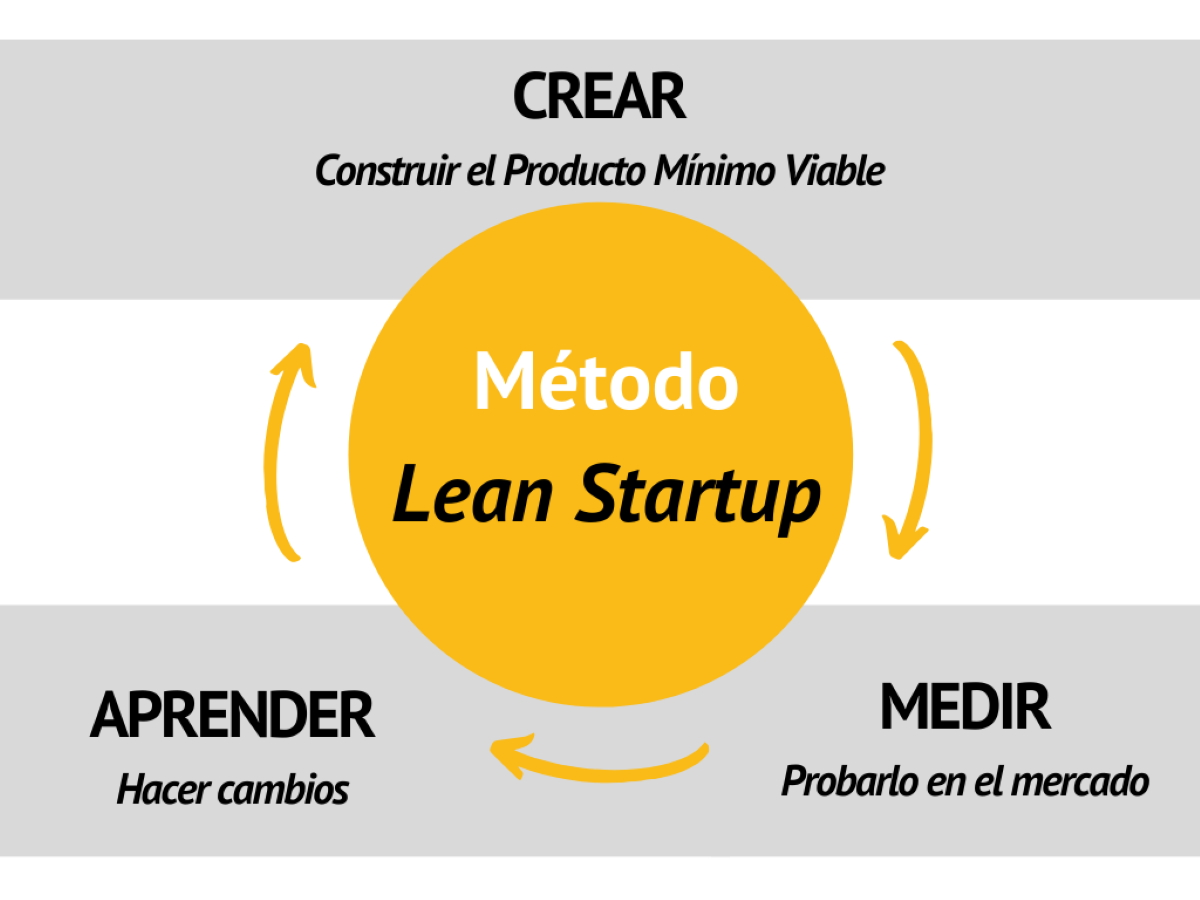
\includegraphics[width=0.7\textwidth]{Images/Infografía-fases-metodología-Lean-Startup.jpg}
          %esto es lo nuevo que agregue
        \fnote{Nota. \textup{Fuente: ¿Qué es el método Lean Startup?}}
\end{minipage}

Mediante este ciclo iterativo y con fundamentos en metodologías ágiles se propone desarrollar negocios en donde los emprendedores basándose en la hipótesis crean un PMV. Este artefacto de desarrollo permite saber con muy poca inversión si la idea desarrollada tiene aceptación en el mercado, cumple y satisface el deseo del cliente y si se tiene capacidad de escalamiento
incrementando funcionalidades o si por el contrario se tiene que tomar acciones para que tome un nuevo enfoque, lo que dentro de este marco de trabajo se considera pivotar.

\subsubsection*{Equipo de trabajo}
En la planeación e implementación de este proyecto estamos conformados por:

\begin{itemize}
    \item \textbf{Gerente general :} encargado de la planeación de las actividades que se desarrollen dentro de la empresa. Organizar los recursos de la entidad. Definir a donde se va a dirigir la empresa en un corto, medio y largo plazo, entre otras muchas tareas. 
    
    \item \textbf{Líder del área de ingeniería :}  responsable de liderar un equipo de desarrollo y responsable de la calidad de sus productos. Establece una visión técnica con el equipo de desarrollo y trabaja con ellos para conseguir el objetivo.
    
    \item \textbf{Director I+D+I :}  El director de I+D+I es responsable del avance tecnológico e investigativo centrados en el avance de la sociedad, siendo una de las partes mas importantes dentro de las tecnologías informativas.
\end{itemize}

\begin{adjustbox}{
            center,
            caption=[{Equipo de trabajo.}]{Equipo de trabajo. },
            label={EquipoDeTrabajo},
            nofloat=table, vspace={20px}}
            \resizebox{\textwidth}{!}{
            \begin{threeparttable}
            \begin{tabular}{|cllll|cllll|}
            \hline
            \multicolumn{5}{|c|}{\cellcolor[HTML]{D9EAD3}Integrante} & \multicolumn{5}{c|}{\cellcolor[HTML]{D9EAD3}Rol}                                          \\ \hline
            \multicolumn{5}{|c|}{Jorge Andres Rojas Bautista}        & \multicolumn{5}{c|}{Gerente general, líder de la área de ingeniería}                      \\ \hline
            \multicolumn{5}{|c|}{Daniela Alexandra Martinez Rueda}   & \multicolumn{5}{c|}{Directora del departamento de investigación, desarrollo e innovación} \\ \hline
            \end{tabular}%
            
            \begin{tablenotes}[para,flushleft]
                \vspace{2mm}
                \textit Nota. Fuente : Autores.
            \end{tablenotes}
            \end{threeparttable} 
            }    
    \end{adjustbox}